\documentclass[12pt]{article}
\usepackage[margin=1in]{geometry}
\usepackage{setspace}
\onehalfspacing{}
\usepackage[dvipsnames,table,xcdraw]{xcolor} % colors

% Start of preamble
%==========================================================================================%
% Required to support mathematical unicode
\usepackage[warnunknown, fasterrors, mathletters]{ucs}
\usepackage[utf8x]{inputenc}

% Standard mathematical typesetting packages
\usepackage{amsmath,amssymb,amscd,amsthm,amsxtra, pxfonts}
\usepackage{mathtools,mathrsfs,xparse}

% Symbol and utility packages
\usepackage{cancel, textcomp}
\usepackage[mathscr]{euscript}
\usepackage[nointegrals]{wasysym}
\usepackage{apacite}

% Extras
\usepackage{physics}  % Lots of useful shortcuts and macros
\usepackage{tikz-cd}  % For drawing commutative diagrams easily
\usepackage{microtype}  % Minature font tweaks
%\usepackage{pgfplots} % plots

\usepackage{enumitem}
\usepackage{titling}

\usepackage{graphicx}

%\usepackage{quiver}

% Fancy theorems due to @intuitively on discord
\usepackage{mdframed}
\newmdtheoremenv[
backgroundcolor=NavyBlue!30,
linewidth=2pt,
linecolor=NavyBlue,
topline=false,
bottomline=false,
rightline=false,
innertopmargin=10pt,
innerbottommargin=10pt,
innerrightmargin=10pt,
innerleftmargin=10pt,
skipabove=\baselineskip,
skipbelow=\baselineskip]{mytheorem}{Theorem}

\newenvironment{theorem}{\begin{mytheorem}}{\end{mytheorem}}

\newtheorem{corollary}{Corollary}
\newtheorem{lemma}{Lemma}

\newtheoremstyle{definitionstyle}
{\topsep}%
{\topsep}%
{}%
{}%
{\bfseries}%
{.}%
{.5em}%
{}%
\theoremstyle{definitionstyle}
\newmdtheoremenv[
backgroundcolor=Violet!30,
linewidth=2pt,
linecolor=Violet,
topline=false,
bottomline=false,
rightline=false,
innertopmargin=10pt,
innerbottommargin=10pt,
innerrightmargin=10pt,
innerleftmargin=10pt,
skipabove=\baselineskip,
skipbelow=\baselineskip,
]{mydef}{Definition}
\newenvironment{definition}{\begin{mydef}}{\end{mydef}}

\newtheorem*{remark}{Remark}

\newtheorem*{example}{Example}
\newtheorem*{claim}{Claim}

% Common shortcuts
\def\mbb#1{\mathbb{#1}}
\def\mfk#1{\mathfrak{#1}}

\def\bN{\mbb{N}}
\def\C{\mbb{C}}
\def\R{\mbb{R}}
\def\bQ{\mbb{Q}}
\def\bZ{\mbb{Z}}
\def\cph{\varphi}
\renewcommand{\th}{\theta}
\def\ve{\varepsilon}
\newcommand{\mg}[1]{\| #1 \|}

% Often helpful macros
\newcommand{\floor}[1]{\left\lfloor#1\right\rfloor}
\newcommand{\ceil}[1]{\left\lceil#1\right\rceil}
\renewcommand{\qed}{\hfill\qedsymbol}
\renewcommand{\ip}[1]{\langle#1\rangle}
\newcommand{\seq}[2]{\qty(#1_#2)_{#2=1}^{\infty}}

\newcommand{\SET}[1]{\Set{\mskip-\medmuskip #1 \mskip-\medmuskip}}

% End of preamble
%==========================================================================================%

% Start of commands specific to this file
%==========================================================================================%

\usepackage{braket}
\newcommand{\Z}{\mbb Z}
\newcommand{\gen}[1]{\left\langle #1 \right\rangle}
\newcommand{\nsg}{\trianglelefteq}
\newcommand{\F}{\mbb F}
\newcommand{\Aut}{\mathrm{Aut}}
\newcommand{\sepdeg}[1]{[#1]_{\mathrm{sep}}}
\newcommand{\Q}{\mbb Q}
\newcommand{\Gal}{\mathrm{Gal}\qty}
\newcommand{\id}{\mathrm{id}}
\newcommand{\Hom}{\mathrm{Hom}_R}
\newcommand{\1}{\mathds 1}
\newcommand{\N}{\mathbb N}
\renewcommand{\P}{\mathbb P \qty}
\newcommand{\E}{\mathbb E \qty}
\newcommand{\Var}{\mathrm{Var}}
\everymath{\displaystyle}
\newcommand{\argmax}{\mathrm{argmax}}
\newcommand{\Area}{\mathrm{Area}}
\usepackage{booktabs}

%==========================================================================================%
% End of commands specific to this file

\title{Math Template}
\date{\today}
\author{Rohan Mukherjee}

\begin{document}
    \maketitle
    \begin{enumerate}
        \item If $f(x,y) = \ip{x,y}$, define $A_{i,j} = \ip{e_i, e_j}$. I then claim that $f(x,y) = x^T Ay$. Writing $x = \sum x_i e_i$ and $y = \sum y_j e_j$, we know that $\ip{x,y} = \sum_{i,j} x_i y_j \ip{e_i,e_j} = \sum_{i,j} x_iy_j A_{i,j} = x^T Ay$ by definition.

        \item The data is as follows:
        \begin{table}[h!]
            \centering
            \begin{tabular}{lccc}
            \toprule
             & \textbf{Smartphones Sold} & \textbf{EV Sales} & \textbf{Social Media Users} \\
            \midrule
            \textbf{Smartphones Sold} & 1.000000 & -0.548806 & -0.297813 \\
            \textbf{EV Sales} & -0.548806 & 1.000000 & 0.888376 \\
            \textbf{Social Media Users} & -0.297813 & 0.888376 & 1.000000 \\
            \bottomrule
            \end{tabular}
            \caption{Correlation Matrix for Smartphones Sold, EV Sales, and Social Media Users.}
            \label{tab:correlation_matrix}
        \end{table}

        Look at that. 0.88 correlation with social media useres with EV sales. That is super surprising.

        \item If there were a magic inner product $\ip{x,y}$ so that $\ip{x,x}_M^{1/2} = \mg{x}_{\ell^3}$, then it would have to be linear, in particular. By some formula whose name I cannot recall:
        \begin{align*}
            4\ip{x,y} = \mg{x+y}_{\ell^3}^2 - \mg{x-y}_{\ell^3}^2. 
        \end{align*}
        Then in particular, the following should hold:
        \begin{align*}
            4\ip{(1,1), (1,2)} &= (2^3 + 3^3)^{2/3} - (1^3)^{2/3} \approx 9.6998 \\
            &= 4\ip{(1,1), (1,0)} + 4\ip{(1,1), (0,2)} \\
            &= (2^3+1^3)^{2/3} - (1^3)^{2/3} + (1^3 + 3^3)^{2/3} - (1^3+1^3)^{2/3} \approx 10.96
        \end{align*}
        This is a contradiction. For higher dimension values, we can just use these same vectors with padded 0s to get the same analysis.


        \item For any configuration of 3 points on the sphere, draw the great circle through them (we may assume they are distinct). Since this is a great circle between 3 points on a sphere of radius 1, the great circle has a radius at most 1. However, if the optimal configuration of the points were to lie on a great circle of radius $<1$, we could have that same configuration with the great circle on the $x$-axis, and this would scale the distances up by a constant factor, making the energy smaller.

        Thus, the optimal point configuration lies on a circle of radius 1. Now there is no need for 3d, we may assume we have put 3 points on the unit circle in $\R^2$. Let the points be named $A,B,C$ and $a,b,c$ the corresponding sidelengths. Then by AM-GM,
        \begin{align*}
            \frac{1}a + \frac1b + \frac1c \geq \frac{3}{\sqrt[3]{abc}}
        \end{align*}
        By circumradius formula, $4R\Area(ABC) = abc$ where $R$ is the circumradius of the triangle formed by ABC. Thus, $abc = 4\Area(ABC)$. This tells us that:
        \begin{align*}
            \frac{1}a + \frac1b + \frac1c \geq \frac{3}{\sqrt[3]{4\Area(ABC)}}
        \end{align*}
        Now we answer the following: among all triangles with circumradius 1, which has the largest area? 
        Draw this triangle on a circle, and label the center of the circle $O$. Connecting all three points to this middle point, we get three triangles. 
        \begin{center}
            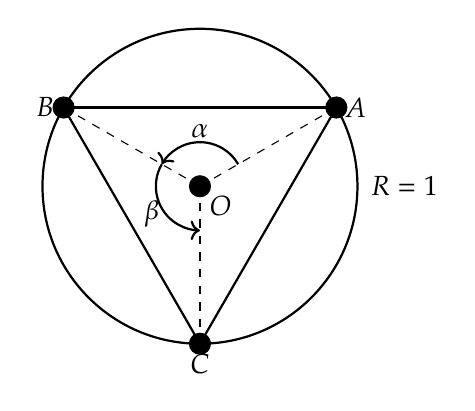
\begin{tikzpicture}[scale=2] % Adjusted scale for better appearance
                % Draw the circle
                \draw[thick] (0,0) circle(1cm);
            
                % Define the points on the circle
                \coordinate (A) at (30:1); % Point A at 30 degrees
                \coordinate (B) at (150:1); % Point B at 150 degrees
                \coordinate (C) at (270:1); % Point C at 270 degrees
                \coordinate (O) at (0,0); % Center of the circle
            
                % Draw the triangle edges
                \draw[thick] (A) -- (B);
                \draw[thick] (B) -- (C);
                \draw[thick] (C) -- (A);
            
                % Draw lines from points to the origin
                \draw[dashed] (A) -- (O);
                \draw[dashed] (B) -- (O);
                \draw[dashed] (C) -- (O);
            
                % Draw the points
                \fill (A) circle(2pt) node[right] {$A$};
                \fill (B) circle(2pt) node[left] {$B$};
                \fill (C) circle(2pt) node[below] {$C$};
                \fill (O) circle(2pt) node[below right] {$O$};
            
                % Add angle labels between the lines
                \draw[->, thick] (30:0.28) arc[start angle=30, end angle=150, radius=0.28];
                \node at (90:0.35) {$\alpha$};
            
                \draw[->, thick] (150:0.28) arc[start angle=150, end angle=270, radius=0.28];
                \node at (210:0.35) {$\beta$};
            
                % Add the circle label
                \node at (1.3,0) {$R=1$};
            \end{tikzpicture}
        \end{center}
        Call the angle between $OA$ and $OB$ $\alpha$, and the angle between $OB$ and $OC$ $\beta$. By the area formula involving sines, $\Area(ABC) = \frac 12 \qty(\sin(\alpha) + \sin(\beta) + \sin(2\pi - \alpha+\beta))$. 

        Now we use Jensen's inequality. $f(x) = \sin(x)$ is concave on $[0,\pi]$, and therefore:
        \begin{align*}
            \frac{\sin(\alpha) + \sin(\beta) + \sin(2\pi - \alpha+\beta)}{3} \leq \sin(\frac{2\pi}{3}) = \frac{\sqrt{3}}{2}
        \end{align*}
        Thus, $\Area(ABC) \leq \frac{3\sqrt{3}}{4}$, with equality being attained when $\alpha = \beta = \frac{2\pi}{3}$. 

        Plugging this back in shows that 
        \begin{align*}
            \frac{1}a + \frac 1b + \frac 1c \geq \frac{3}{\sqrt[3]{4 \cdot (3\sqrt{3}/4)}} = \sqrt{3}. 
        \end{align*}
        with equality iff the triangle is equilateral, i.e. $a = b = c$. It is then easy to see that the points $(1, 0)$, $\qty(-\frac 12, \frac{\sqrt{3}}{2})$, and $\qty(-\frac 12, -\frac{\sqrt{3}}{2})$ sate this bound.
    \end{enumerate}
\end{document}